\chapter{The Zeta Function of Riemann (Contd).}\label{chap11}

\setcounter{section}{2}
\section[Analytic continuation of $\zeta(s)$. First
  method]{Analytic continuation of {\boldmath$\zeta(s)$}. First
  method \cite[p.18]{key16}}\label{chap11:sec3}\pageoriginale 

We have, for $\sigma >0$,
$$
\Gamma (s) = \int\limits^\infty_{0} x^{s-1} e^{-x} dx.
$$
Writing $nx$ for $x$, and summing over $n$, we get
\begin{align*}
\sum\limits^\infty_{n=1} \frac{\Gamma(s)}{n^s} & = \sum^\infty_{n=1}\;
\int\limits^\infty_{n=0} x^{s-1} e^{-nx} dx\\
& = \int\limits^\infty_0 \left(\sum\limits^\infty_{n=1} e^{-nx}
\right) x^{s-1} dx, \text{ if } \sigma >1.
\end{align*}
since 
$$
\sum\limits^\infty_{n=1} \left|\int\limits^\infty x^{s-1} e^{-nx} dx
\right| \leq \sum\limits^\infty_{n=1} \int\limits^\infty_0 x^{\sigma
  -1} e^{-nx} dx = \sum\limits^\infty_{n=1}
\frac{\Gamma(\sigma)}{n^\sigma} < \infty,
$$
if $\sigma >1$. Hence
$$
\sum\limits^\infty_{n=1} \frac{\Gamma(s)}{n^s} = \int\limits^\infty_0
\frac{e^{-x}}{1-e^{-x}}  x^{s-1} dx = \int\limits^\infty_0
\frac{x^{s-1}dx}{e^x -1} 
$$
or
$$
\text{\fbox{$\Gamma(s)\zeta(s) = \int\limits^\infty_{0}
    \dfrac{x^{s-1}}{e^{x}-1} dx , \;\; \sigma >1$}}  
$$

In order to continue $\zeta(s)$ analytically all over the $s$-plane,
consider the complex integral
$$
I(s) = \int\limits_C \frac{z^{s-1}}{e-1} dz
$$
where $C$ is a contour consisting of the real axis from $+ \infty$ to
$\rho$, $0< \rho < 2 \pi$, the circle\pageoriginale $|z| = \rho$; and
the real axis from $\rho$ to $\infty$. $I(s)$, if convergent, is
independent of $\rho$, by {\em Cauchy's} theorem.

Now, on the circle $|z| = \rho$, we have
\begin{align*}
|z^{s-1}| = |e^{(s-1)\log z}| & =|e^{\{(\sigma -1) + it\}\{\log |z| +
  i \arg z\} }| \\
& = e^{(\sigma -1) \log |z| - t \arg z }\\
& = |z|^{\sigma-1} e^{2\pi |t|},
\end{align*}
while
$$
|e^z-1| >  A|z|;
$$
Hence, for fixed $s$, 
$$
\left|\;\int\limits_{|z|=\rho}\right| \leq \frac{2\pi \rho \cdot 
  \rho^{\sigma-1}}{A\rho} \cdot e^{2\pi|t|} \to 0 \text{ as } \rho  \to 
0, \text{ if } \sigma > 1.
$$

Thus, on letting $\rho \to 0$, we get, if $\sigma >1$,
\begin{align*}
I(s) & = -\int\limits^\infty_0 \frac{x^{s-1}}{e^x-1} dx +
\int\limits^\infty_0 \frac{(xe^{2\pi i})^{s-1}}{e^x-1} \, dx\\
& = - \Gamma (s)  \zeta (s) + e^{2\pi is} \Gamma (s) \zeta (s)\\
& = \Gamma (s) \zeta(s) (e^{2\pi is} -1).
\end{align*}

Using the result
$$
\Gamma(s) \Gamma(1-s) = \frac{\pi}{ \sin \pi s}
$$
we get\pageoriginale
\begin{align*}
I(s) & = \frac{\zeta(s)}{\Gamma(1-s)} \cdot 2 \pi i \cdot \frac{e^{2\pi i
    s}-1}{e^{\pi i s} - e^{-\pi i s}}\\
& = \frac{\zeta(s)}{\Gamma(1-s)} \cdot 2 \pi i \cdot e^{\pi i s},
\end{align*}
or 
$$
\text{\fbox{$\zeta (s) = \dfrac{e^{-i\pi s} \Gamma (1-s)}{2\pi i}
    \int\limits_C \dfrac{z^{s-1}}{e^z-1}dz\,, \; \; \sigma >1.$}} 
$$
The integral on the right is uniformly convergent in any finite region
of the $s$-plane (by obvious majorization of the integrand), and so
defines an entire function. Hence the above formula, proved first for
$\sigma >1$, defines $\zeta(s)$, as a meromorphic function, all over
the $s$-plane. This only possible poles are the poles of
$\Gamma(1-s)$, namely $s = 1, 2, 3, \ldots$. We know that $\zeta(s)$
is regular for $s = 2,3, \ldots$ (As a matter of fact, $I(s)$ vanishes
at these points). Hence the only possible pole is at $s =1$.

Hence
$$
I(1) = \int\limits_{C} \frac{dz}{e^z-1} = 2 \pi i,
$$
while
$$
\Gamma (1-s) = - \frac{1}{s-1} +\cdots
$$
Hence \textit{the residue of $\zeta(s)$ at $s=1$ is $1$}.

We see in passing, since 
$$
\frac{1}{e^z-1} = \frac{1}{z} - \frac{1}{2} + B_1 \frac{z}{2!} - B_2
\frac{z^3}{4!} + \cdots 
$$\pageoriginale
that
$$
\zeta(0) = - \frac{1}{2}, \zeta(-2m) =0, \zeta(1-2m) = \frac{(-1)^m
  B_m}{2m} , m = 1,2,3,\ldots 
$$

\section[Functional Equation (First method)]{Functional Equation (First method) \cite[p.18]{key16}}\label{chap11:sec4}

Consider the integral
$$
\int \frac{z^{s-1}}{e^z -1}dz
$$
taken along $C_n$ as in the diagram. 

\begin{figure}[H]
\centering
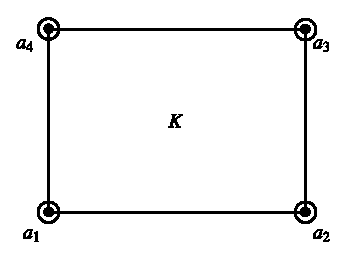
\includegraphics{figures/fig11.1.eps}
\end{figure}

Between $C$ and $C_n$, the integrand has poles at 
$$
\pm 2i \pi, \ldots, \pm 2 n i \pi. 
$$
The residue at 
$$2m\pi i \mbox{ is } (2 m \pi e^{\frac{\pi}{2} i})^{s-1}$$ 
while the residue at $-2m\pi i$ is $(2m\pi e^{3/2 \pi i})^{s-1}$; taken together
they amount to
\begin{align*}
& (2m \pi) e^{\pi i (s-1)} \left[e^{\frac{\pi i}{2} (s-1)} +
    e^{-\frac{\pi i}{2}(s-1)} \right]  \\
& = (2m\pi)^{s-1} e^{\pi i (s-1)} 2 \cos \left(\frac{\pi}{2} (s-1)\right)\\
& = -2 (2m \pi)^{s-1} e^{\pi i s} \sin \left(\frac{\pi}{2} s\right) 
\end{align*}
Hence\pageoriginale
$$
I(s) = \int\limits_{C_n} \frac{z^{s-1}}{e^z-1}dz + 4 \pi i \sin
\left(\frac{\pi s}{2}\right) e^{\pi i s} \sum\limits^n_{m=1} (2m \pi)^{s-1}
$$
by the theorem of residues.

Now let $\sigma <0$, and $n \to \infty$. Then, on $C_n$,
$$
|z^{s-1}| = O (|z|^{\sigma-1}) = O(n^{\sigma-1}),
$$
and
$$
\frac{1}{e^z-1} = O(1),
$$
for
\begin{align*}
|e^z-1|^2 = |e^{x+iy} -1|^2 & =  |e^x (\cos y + i \sin y )-1|^2\\
& = e^{2x} - 2 e^x \cos y + 1,
\end{align*}
which, on the vertical lines, is $ \geq (e^x -1)^2$ and, on the
horizontal lines, $=(e^x +1)^2$. (since $\cos  y = -1$ there).

Also the length of the square-path is $O(n)$. Hence the integral round
the square $\to 0$ as $n \to \infty$.

Hence
\begin{align*}
I(s) & = 4 \pi i e^{\pi i s} \sin\left(\frac{\pi s}{2}\right)
\sum\limits^\infty_{m=1} (2m \pi)^{s-1}\\
& = 4 \pi i e^{\pi i s} \sin \left(\frac{\pi s}{2}\right) \cdot (2\pi)^{s-1} \zeta
(1-s), \text{ if } \sigma < 0. 
\end{align*}
or\pageoriginale
\begin{align*}
\zeta(s) \Gamma (s) (e^{2\pi is}-1) & = (4\pi i) (2\pi)^{s-1} e^{\pi i
s} \sin \left(\frac{\pi s}{2}\right) \zeta(1-s)\\
& = 2 \pi i e^{\pi i s} \frac{\zeta(s)}{\Gamma(1-s)}
\end{align*}

Thus
$$
\text{\fbox{$\zeta(s) = \Gamma (1-s) \zeta(1-s) 2^s \pi^{s-1}
    \sin\left(\dfrac{\pi s}{2}\right)$,}}
$$
for $\sigma < 0$, and hence, by analytic continuation, for all values
of $s$ (each side is regular except for poles!).

This is the functional equation.

Since
$$
\Gamma \left(\frac{x}{2} \right) \Gamma \left(\frac{x+1}{2} \right) =
\frac{\sqrt{\pi}}{2^{x-1}} \Gamma(x),
$$
we get, on writing $x=1-s$, 
$$
2^{-s} \Gamma \left( \frac{1-s}{2}\right) \Gamma \left(1-\frac{s}{2}
\right) = \sqrt{\pi} \Gamma (1-s);
$$
also 
$$
\Gamma \left(\frac{s}{2} \right) \Gamma \left(1-\frac{s}{2} \right) =
\frac{\pi}{\sin \left(\frac{\pi s}{2}\right)} 
$$
Hence
$$
\Gamma(1-s) = 2^{-s} \Gamma \left(\frac{1-s}{2} \right) \left\{\Gamma
\left(\frac{s}{2} \right) \right\}^{-1} \sqrt{\pi} \left\{\sin\left(\frac{\pi
  s}{2}\right)\right\}^{-1} 
$$
Thus
$$
\text{\fbox{$\pi^{-s/2} \Gamma(s/2) \zeta(s) = \pi^{-\frac{(1-s)}{2}}
\Gamma \left(\dfrac{1-s}{2} \right)\zeta(1-s) $}} 
$$
If\pageoriginale
\begin{align*}
\xi (s) & \equiv \frac{1}{2} s(s-1) \pi^{-s/2} \Gamma(s/2) \zeta(s)\\
& \equiv \frac{1}{2} s(s-1) \eta(s),
\end{align*}
then $\eta(s) = \eta(1-s)$ and $\xi (s) = \xi (1-s)$. If $\equiv (z) =
\xi \left(\frac{1}{2} + iz\right)$, then $\equiv (z) \equiv (-z)$.

\section[Functional Equation (Second Method)]{Functional Equation (Second Method) \cite[p.13]{key16}}\label{chap11:sec5}
Consider the lemma given in Lecture \ref{chap9}, and write $\lambda_n =n$, $a_n
=1$, $\phi(x) = x^{-s}$ in it. We then get
\begin{align*}
\sum\limits_{n \leq x} n^{-s} & = s \int\limits^X_1 \frac{[x]}{x^{s+1}}
dx + \frac{[X]}{X^s} , \text{ if } X \geq 1.\\
& = \frac{s}{s-1} -\frac{s}{(s-1)X^{s-1}}  - s \int\limits^X_1
\frac{x-[x]}{x^{s+1}} dx + \frac{1}{X^{s-1}} - \frac{X-[X]}{X^s}
\end{align*}
Since
$$
\left|\frac{1}{X^{s-1}} \right| = \frac{1}{X^{\sigma-1}} , \text{ and } \left|
\frac{X-[X]}{X^s} \leq \frac{1}{X^\sigma},
\right|
$$
we deduce, on making $X \to \infty$,
$$
\text{\fbox{$\zeta(s) = \frac{s}{s-1} - s \int\limits^\infty_1
    \frac{x-[x]}{x^{s+1}} dx, $ if $\sigma > 1$}}
$$
or
\begin{equation}
\text{\fbox{$\zeta(s) = s \int\limits^\infty_1
    \frac{[x]-x+\frac{1}{2}}{x^{s+1}} dx + \frac{1}{s-1} +
    \frac{1}{2}$, if $\sigma > 1$}}\label{chap11:subsec5.1}
\end{equation}

 Since\pageoriginale $[x] - x + \dfrac{1}{2}$ is bounded, the
integral on the right hand side converges for $\sigma >0$, and
uniformly in any finite region to the right of $\sigma =0$. Hence it
represents an analytic function of $s$ \textit{regular for $\sigma
  >0$}, and so provides the continuation of $\zeta(s)$ up to $\sigma
=0$, and $s=1$ is clearly a simple pole with residue $1$.

For $0 < \sigma < 1$, we have, however, 
$$
\int\limits^1_0 \frac{[x] -x}{x^{s+1}} dx = - \int\limits^1_0 x^{-s}
dx = \frac{1}{s-1}, 
$$
and 
$$
\frac{s}{2} = \int\limits^\infty_1 \frac{dx}{x^{s+1}} = \frac{1}{2} 
$$
Hence

\begin{equation}
\zeta(s) = s \int\limits^\infty_0 \frac{[x] - x}{x^{s+1}} dx, \quad 0
<  \sigma < 1\label{chap11:subsec5.2}
\end{equation}

We have seen that (\ref{chap11:subsec5.1}) gives the analytic continuation up to $\sigma 
=0$. By refining the argument dealing with the integral on the
right-hand side of (\ref{chap11:subsec5.1}) we can get the continuation all over the
$s$-plane. For, if 
$$
f(x) \equiv [x] - x + \frac{1}{2} , \quad f_1 (x) \equiv
\int\limits^x_1 f(y) dy,
$$
then $f_1(x)$ is \textit{also} bounded, since  $\int\limits^{n+1}_n
  f(y) dy =0$ for any integer $n$.


Hence\pageoriginale
\begin{gather*}
\left. \int\limits^{x_2}_{x_1} \frac{f(x)}{x^{s+1}}
dx = \frac{f_1(x)}{x^{s+1}}\right]^{x_2}_{x_1} + (s+1) \int\limits^{x_2}_{x_1}
  \frac{f_1(x)}{x^{s+2}} dx\\
\to 0, \text{ as } x_1 \to \infty , x_2 \to \infty, \\
\text{\fbox{if $\sigma > -1$.}}
\end{gather*}

Hence the integral in (\ref{chap11:subsec5.1}) converges for $\sigma > - 1$. 

Further
\begin{align}
&s \int\limits^1_0 \frac{[x] -x + \frac{1}{2}}{x^{s+1}} dx =
\frac{1}{s-1} + \frac{1}{2}, \text{ for } \sigma < 0;\notag\\
&\text{\fbox{$\zeta(s) = s \int\limits^\infty_0 \frac{[x] - x +
      \frac{1}{2}}{x^{s +1}} dx, \;\; -1 < \sigma < 0$}}
\label{c11:eq5.3}
\end{align}

Now the function $[x] - x + \frac{1}{2}$ has the Fourier expansion
$$
\sum\limits^\infty_{n=1} \frac{\sin 2n \pi x}{n \pi}
$$
if $x$ is \textit{not} an integer. The series is boundedly
convergent. If we substitute it in (\ref{c11:eq5.3}), we get
\begin{align}
\zeta(s) & = \frac{s}{\pi} \sum\limits^\infty_{n=1} \frac{1}{n}
\int\limits^\infty_0 \frac{\sin 2n \pi  x}{x^{s+1}} dx\notag\\
& = \frac{s}{\pi} \sum\limits^\infty_{n=1} \frac{(2n\pi)^s}{n}
\int\limits^\infty_0 \frac{\sin y}{y^{s+1}} dy\notag\\
\zeta(s) & = \frac{s}{\pi} (2\pi)^s \{-\Gamma (1-s)\} \sin
\frac{s\pi}{2} \zeta(1-s),\label{chap11:subsec5.4}
\end{align}

If\pageoriginale term wise integration is permitted, \textit{for
  $-1<\sigma   <0$}. The right hand side is, however, analytic for all
values of $s$ such that $\sigma < 0$. Hence (\ref{chap11:subsec5.4}) provides the analytic
continuation (not only for $-1< \sigma <0$) all over the $s$-plane. 

The term-wise integration preceding (\ref{chap11:subsec5.4}) is certainly justified over
any \textit{finite} range since the concerned series is boundedly
convergent. We have therefore only to prove that
$$
\lim\limits_{X \to \infty} \sum\limits^\infty_{n=1} \frac{1}{n}
\int\limits^\infty_X \frac{\sin 2n \pi x}{x^{s+1}} dx = 0, -1 < \sigma <0
$$
Now
\begin{align*}
\int\limits^\infty_X \frac{\sin 2 n \pi x}{x^{s+1}} dx & =
\left[-\frac{\cos 2n \pi x}{2n \pi x^{s+1}} \right]^\infty_X -
\frac{s+1}{2n \pi} \int\limits^\infty_X \frac{2n \pi x}{x^{s+2}} dx \\
& = O \left(\frac{1}{nX^{\sigma+1}} \right) + O \left(\frac{1}{n}
\int\limits^\infty_X \frac{dx}{x^{\sigma+2}} \right) \\
& = O \left(\frac{1}{nX^{\sigma+1}} \right)
\end{align*}
and hence
$$
\lim\limits_{X \to \infty} \sum\limits^\infty_{n=1} \frac{1}{n}
\int\limits^\infty_X \frac{\sin 2n \pi x}{x^{s+1}} dx = 0,\text{ if }
-1 < \sigma < 0
$$

This completes the analytic continuation and the proof of the
Functional equation by the second method.

As a consequence of (\ref{chap11:subsec5.1}), we get
\begin{align*}
\lim\limits_{s\to 1} \left\{\zeta (s) - \frac{1}{s-1} \right\} & =
\int\limits^\infty_1 \frac{[x]-x+\frac{1}{2}}{x^2} dx + \frac{1}{2}\\
& = \lim\limits_{n\to \infty} \int\limits^n_1 \frac{[x]-x}{x^2} dx
+1\\
& = \lim\limits_{n \to \infty} \left\{\sum\limits^{n-1}_{m=1} m
\int\limits^{m+1}_m \frac{dx}{x^2} - \log n +1 \right\}\\
& = \lim\limits_{n \to \infty} \left\{\sum\limits^{n-1}_{m=1}
\frac{1}{m+1} + 1 - \log n  \right\}\\
& = \gamma
\end{align*}\pageoriginale

Hence, near $s=1$, we have
$$
\zeta(s) = \frac{1}{s-1} + \gamma + O (|s-1|).
$$

